\documentclass[11pt,a4paper]{article}

% Pacchetti fondamentali
\usepackage[utf8]{inputenc}
\usepackage[italian]{babel}
\usepackage{amsmath}
\usepackage{graphicx}
\usepackage{geometry}
\usepackage{booktabs}
\usepackage{float}
\usepackage{hyperref}
\usepackage{caption}
\usepackage{longtable}

% Margini del testo ripristinati a 2.5cm (standard accademico)
\geometry{a4paper, top=2.5cm, bottom=2.5cm, left=2.5cm, right=2.5cm}

\title{\textbf{Analisi delle Prestazioni di Modelli Centralizzati ILP per il Task Routing}}
\author{Claudio Bagini 2045337}
\date{\today}

\begin{document}

\maketitle

\section{Introduzione}
Nel contesto dei sistemi distribuiti moderni e dell'edge computing, l'allocazione efficiente delle risorse computazionali (Resource Allocation) e l'istradamento dei task (Task Routing) rappresentano sfide critiche e di primaria importanza. 

Il sistema analizzato in questo studio sfrutta un approccio centralizzato basato su Integer Linear Programming (ILP) per mappare le richieste in ingresso sui nodi server disponibili. A differenza delle euristiche, che compiono scelte ottime a livello puramente locale (ma spesso sub-ottime a livello globale), il modello ILP garantisce l'individuazione di una soluzione matematicamente perfetta per un dato set di richieste.

Per comprendere a fondo l'impatto delle policy di orchestrazione e il comportamento del solutore centralizzato sotto stress, il modello è stato testato imponendo due diverse strategie di mappatura (\textit{Objective Mapping}) nella funzione obiettivo:
\begin{itemize}
    \item \textbf{Mapping Time:} I pesi della funzione obiettivo privilegiano la minimizzazione del tempo totale di risposta e di trasmissione ($W_{lat}=1, W_{en}=0$). Questa strategia è cruciale per i servizi altamente sensibili al ritardo (delay-sensitive).
    \item \textbf{Mapping Energy:} I pesi della funzione obiettivo privilegiano il risparmio energetico dei nodi e della rete ($W_{lat}=0, W_{en}=1$), parametro fondamentale per estendere la vita operativa di infrastrutture con rigidi vincoli di power-budget.
\end{itemize}
Le simulazioni mirano a individuare i colli di bottiglia fisici e logici del sistema e a valutare quali configurazioni di \textit{Batch Size} (dimensione della coda di richieste aggregata) e \textit{Batch Timeout} (tempo massimo di attesa prima di innescare l'ILP) garantiscano la maggiore resilienza al variare del tasso di arrivo delle richieste nella rete.

\section{Setup Sperimentale}
Le simulazioni sono state eseguite mantenendo un set di parametri di base costanti (ispirati al paper ICDCS di riferimento), al fine di isolare l'impatto delle metriche di interesse.

\subsection{Parametri e Variabili dell'Esperimento}
\begin{itemize}
    \item \textbf{Budget Energetico Globale:} Fissato rigorosamente a 80 KJ per l'intera durata di ogni iterazione di simulazione.
    \item \textbf{Arrival Rate (Carico di Rete):} Variabile indipendente principale. Il tasso di arrivo delle richieste è stato modulato per simulare scenari di traffico progressivo: da 2, 3, 4, 6, 8 fino a 10 richieste al secondo. Nel motore del simulatore, questi valori corrispondono a tempi di inter-arrivo (\textit{AT}) decrescenti (da $0.5$ a $0.1$ secondi).
    \item \textbf{Configurazioni di Batching:} Per ogni livello di \textit{Arrival Rate}, sono state testate molteplici configurazioni incrociate. Variando la \textit{Batch Size} (BS), si è stabilito quante richieste accumulare prima di avviare il solutore ILP (da 1 a 20). Variando il \textit{Batch Timeout} (BT), si è imposto un limite temporale massimo per prevenire lo stallo delle richieste (starvation) in scenari di traffico rado.
    \item \textbf{Coefficienti di Ponderazione ($\alpha$, $\beta$, $\gamma$):} In stretta conformità con il modello matematico del paper di riferimento, i vettori dei pesi che regolano i trade-off e i costi delle risorse all'interno della formulazione ILP sono stati mantenuti costanti, garantendo la coerenza dell'esperimento. Nello specifico, i parametri di profilazione sono stati fissati ai seguenti valori vettoriali: $\alpha = (0.3, 0.5, 0.2)$, $\beta = (0.4, 0.35, 0.25)$ e $\gamma = (0.7, 0.3)$.
\end{itemize}


\section{Migliorie e Correzioni Apportate}
In questa sezione vengono illustrate sinteticamente le principali modifiche apportate al simulatore. Gli interventi hanno riguardato sia l'introduzione di nuove funzionalità volte a ottimizzare le prestazioni del sistema, sia la risoluzione di anomalie critiche riscontrate nella gestione dei task e nel calcolo delle metriche prestazionali.

\begin{itemize}
    \item \textbf{Implementazione del Load Balancer:} È stata introdotta una logica di bilanciamento del carico con l'obiettivo di distribuire in modo efficiente ed equo le richieste tra i server disponibili. Questo intervento ha permesso di ridurre i colli di bottiglia e di minimizzare i tassi di rifiuto causati dalla saturazione delle singole risorse di calcolo.
    
    \item \textbf{Implementazione del meccanismo di Retry ILP:} Per far fronte ai casi in cui il modello di Programmazione Lineare Intera (ILP) restituisca un problema non ammissibile (\textit{infeasible}), è stata integrata una logica di retry. 
    
    \item \textbf{Implementazione del Fallback Greedy per l'Uplink:} Al fine di garantire la resilienza del sistema, è stato integrato un'approccio di tipo \textit{greedy} che agisce come strategia di ripiego (\textit{fallback}) per la fase di uplink, qualora il path deciso dall'ILP venisse iterrotto a causa degli spostamenti orbitali.
    
    \item \textbf{Implementazione della logica di Sunset:} È stata introdotta una gestione formale degli eventi di \textit{sunset}, volta a favorire i SEN che non oltrepassano la soglia del range di comunicazione.
    
    \item \textbf{Fix della logica di Uplink dei Task:} È stato risolto un bug critico nella fase di trasmissione verso l'alto (\textit{uplink}) dei task. La correzione ha sanato le anomalie nell'assegnazione delle rotte di rete e nel rispetto dei vincoli di larghezza di banda, garantendo una corretta propagazione dei dati verso i nodi di elaborazione.
    
    \item \textbf{Fix del calcolo del \textit{Time in System}:} È stata corretta ed estesa la formula per la misurazione del tempo totale trascorso da un task all'interno del sistema. Il nuovo calcolo include ora in modo preciso ed esaustivo tutte le componenti temporali, tracciando correttamente i tempi di attesa nei batch (\textit{wait time}), i ritardi di rete e il tempo effettivo di esecuzione (\textit{system execution}).
\end{itemize}

\section{Analisi dei Risultati}
Di seguito vengono presentati e discussi i risultati per le tre metriche cardine: Success Rate, Cause di Rigetto e Response Time.

\subsection{Success Rate (Tasso di Completamento)}
Il tasso di successo rappresenta la percentuale di task che sono stati correttamente presi in carico, elaborati e restituiti all'utente senza violare la deadline e il budget energetico.

\begin{figure}[H]
    % \makebox e 1.15\textwidth permettono all'immagine di espandersi oltre i margini del testo!
    \makebox[\textwidth][c]{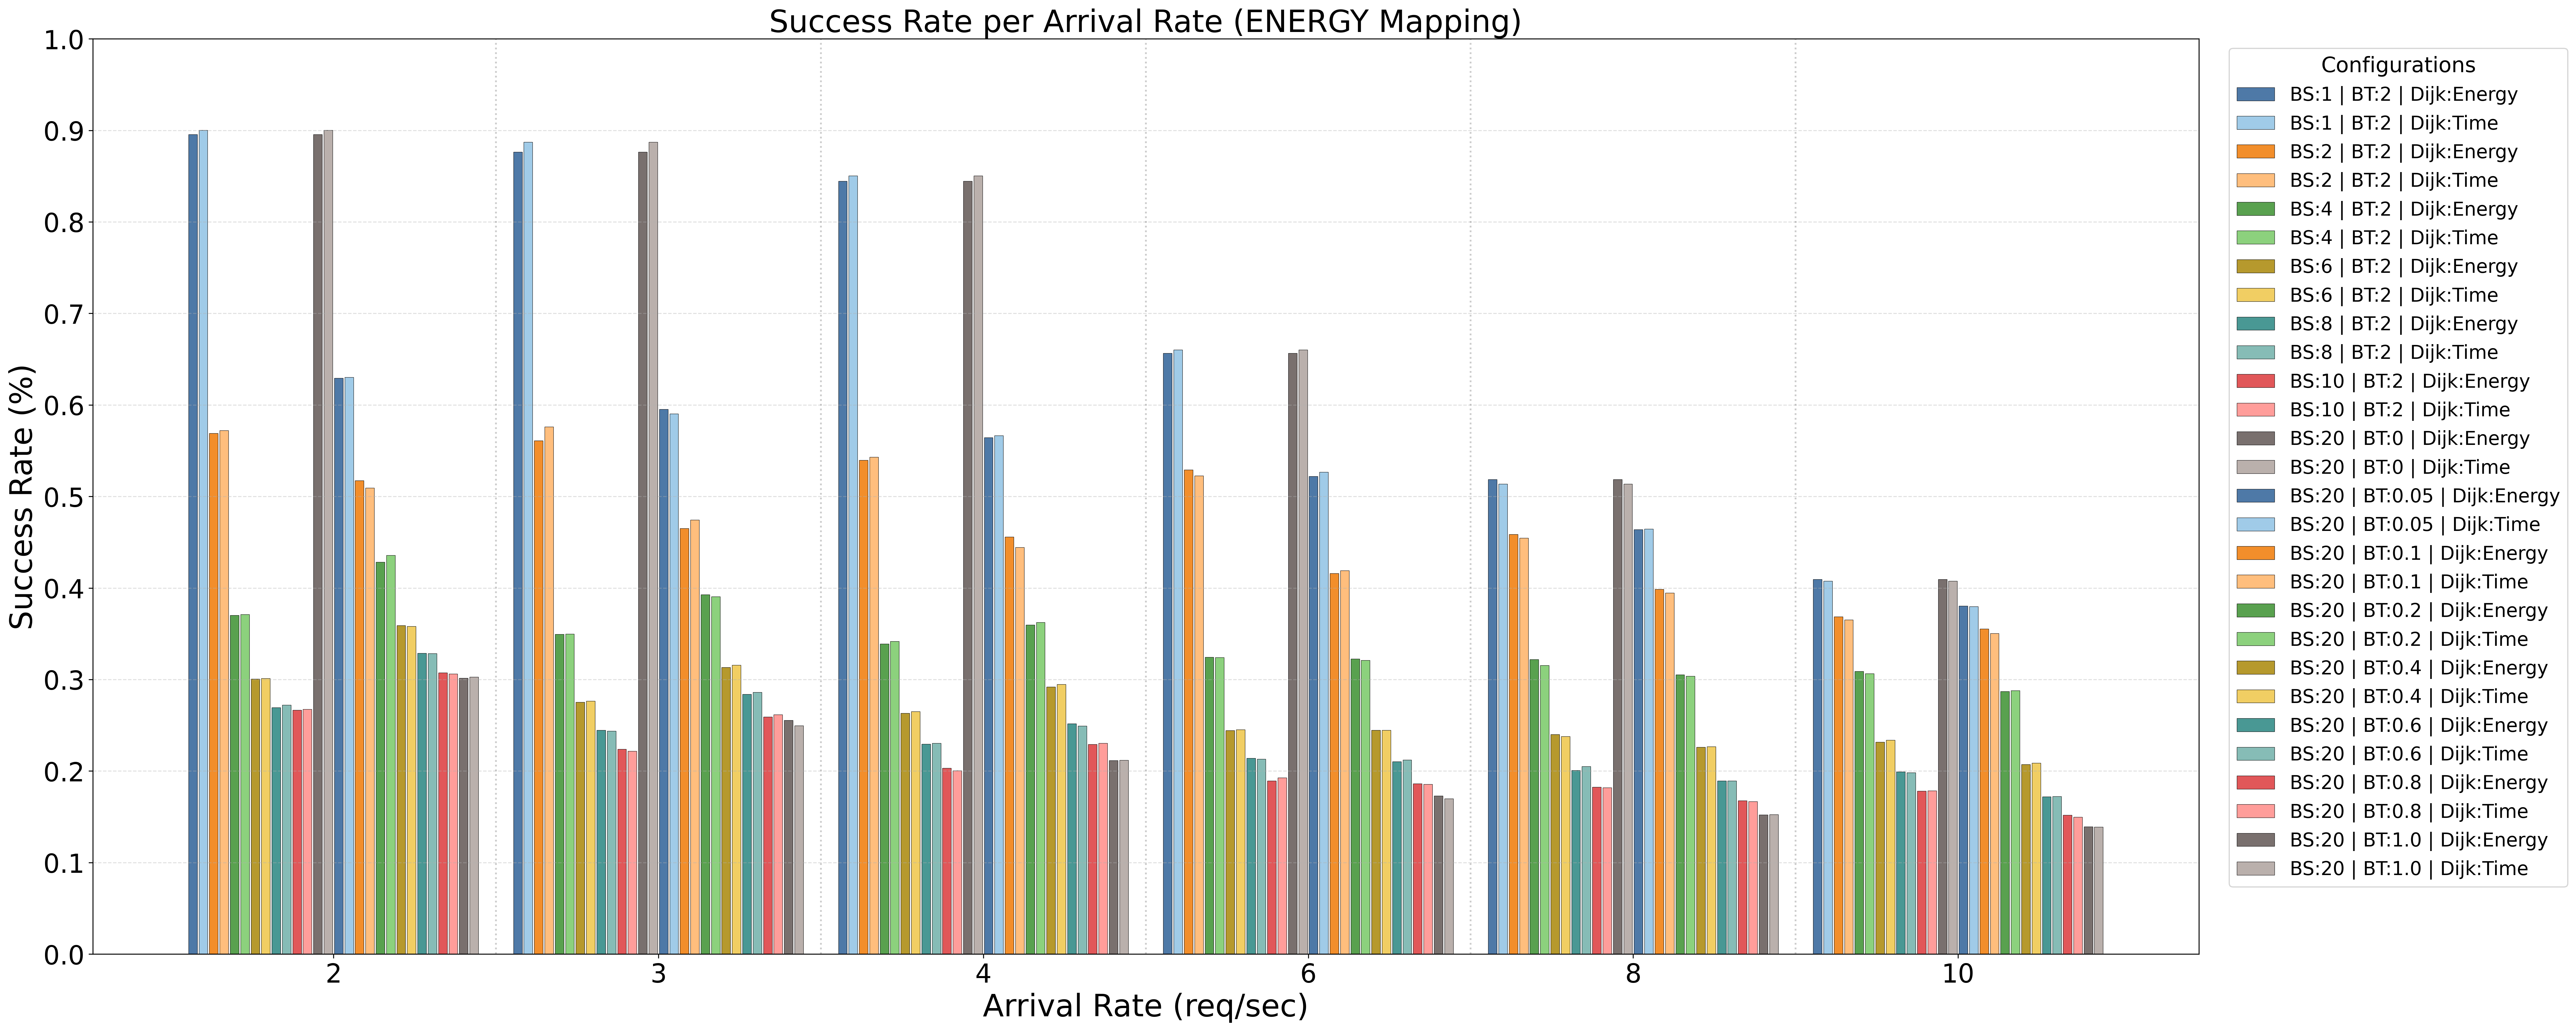
\includegraphics[width=1.3\textwidth]{01_AR_success_rate_energy.png}}
    \caption{Success Rate - Configurazione Energy.}
    \label{fig:suc_energy}
\end{figure}

\begin{figure}[H]
    \makebox[\textwidth][c]{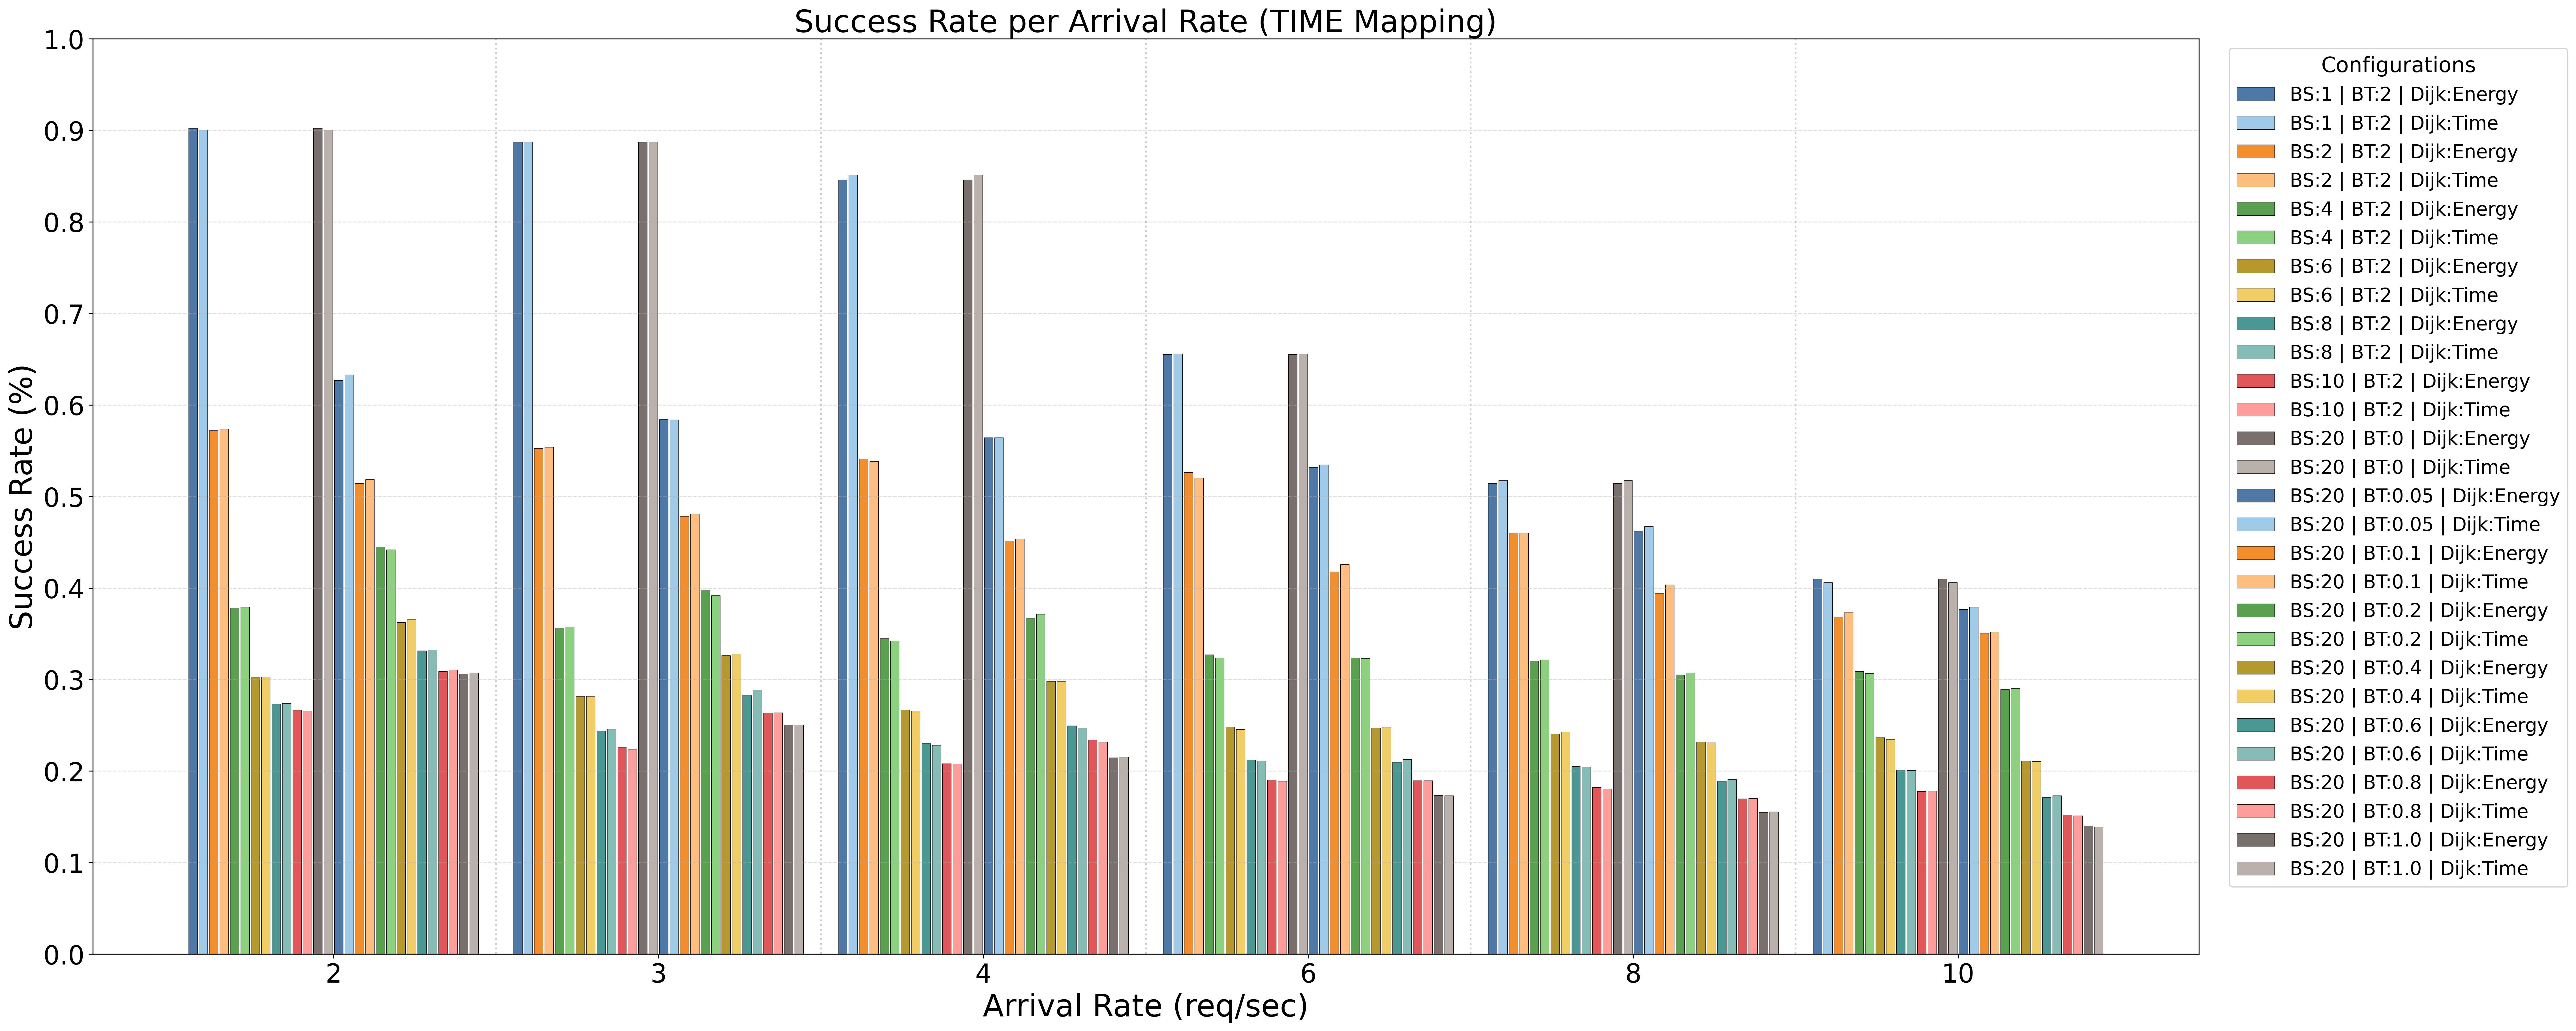
\includegraphics[width=1.3\textwidth]{01_AR_success_rate_time.png}}
    \caption{Success Rate - Configurazione Time.}
    \label{fig:suc_time}
\end{figure}

All'aumentare dell'Arrival Rate (da 2 a 10~req/sec), le prestazioni del sistema subiscono un marcato degrado: il tasso di successo crolla infatti da picchi del 90\% a valori inferiori al 40\% (Figure~\ref{fig:suc_energy} e~\ref{fig:suc_time}). 

I nuovi scenari evidenziano che le configurazioni senza aggregazione ($BS=1$) o con tempo di attesa nullo ($BS=20$ con $BT=0$) mantengono le percentuali di successo nettamente più elevate. L'analisi dimostra che il vero collo di bottiglia prestazionale non è l'ampiezza del batch in sé, bensì il ritardo introdotto per riempirlo. 

Osservando le configurazioni con $BS=20$, si nota come all'aumentare del Batch Timeout ($BT$ da 0.05 a 1.0) i risultati precipitino, eguagliando le scarse prestazioni dei batch staticamente ampi (es. $BS=8$ o $10$). L'attesa forzata per aggregare le richieste ne penalizza quindi irreversibilmente i tempi utili per l'accettazione. Infine, questa dinamica comportamentale si conferma identica sia ottimizzando l'instradamento per \textit{Time} che per \textit{Energy}.

\subsection{Analisi delle Cause di Rigetto (Rejection Causes)}
Per diagnosticare con esattezza la causa del collasso prestazionale, i task scartati sono stati analizzati in base allo stato di fallimento registrato.

\begin{figure}[H]
    \makebox[\textwidth][c]{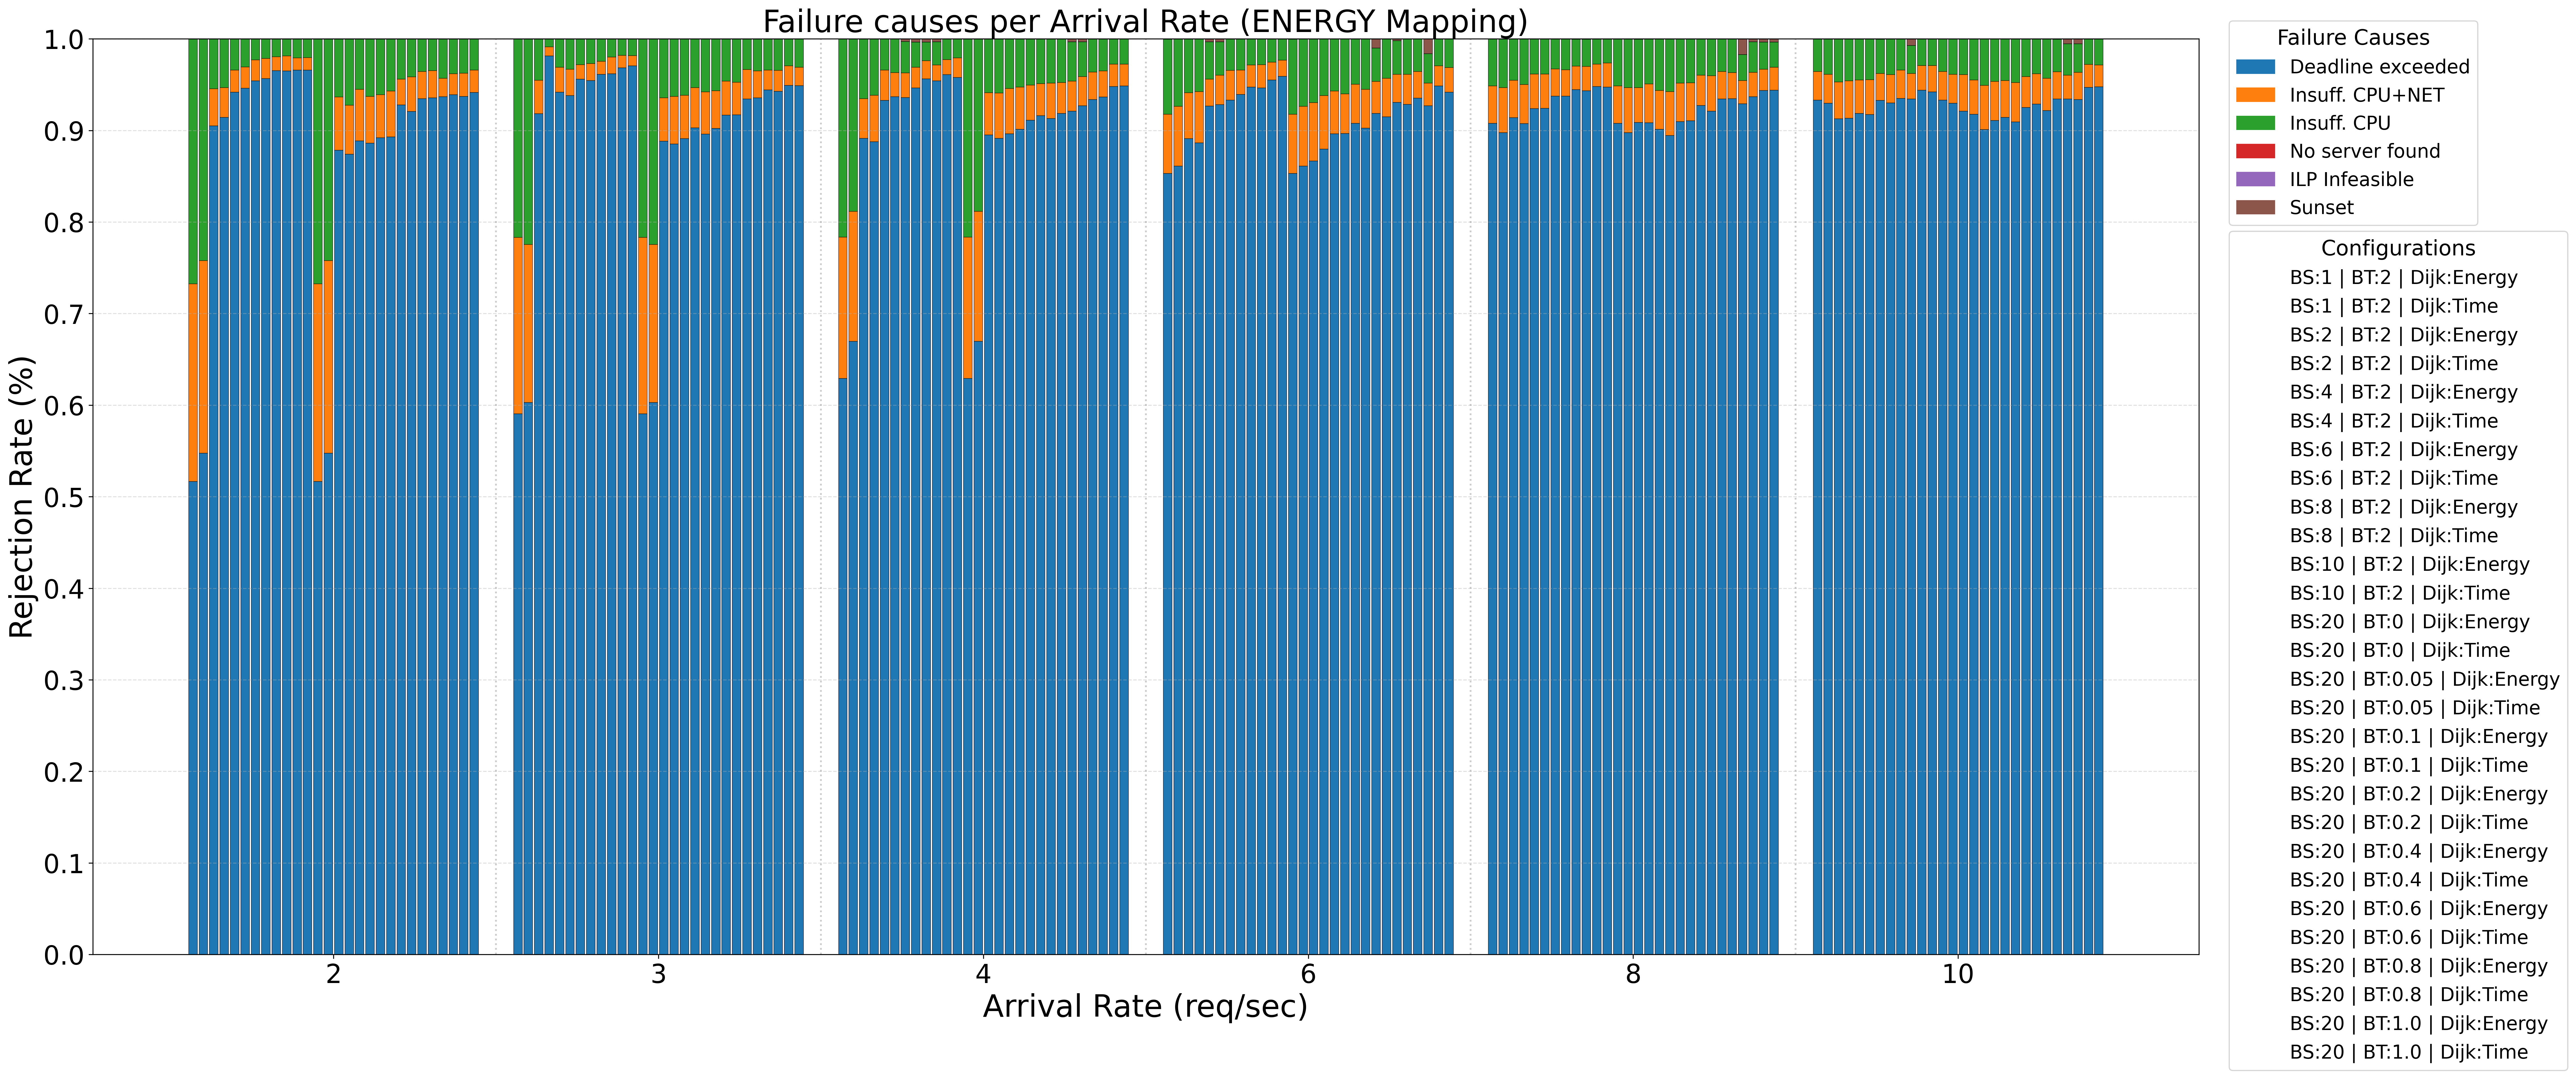
\includegraphics[width=1.3\textwidth]{02_AR_rejection_energy.png}}
    \caption{Distribuzione delle Cause di Rigetto sul totale dei task (Configurazione Energy).}
        \label{fig:rej_energy}
\end{figure}

\begin{figure}[H]
    \makebox[\textwidth][c]{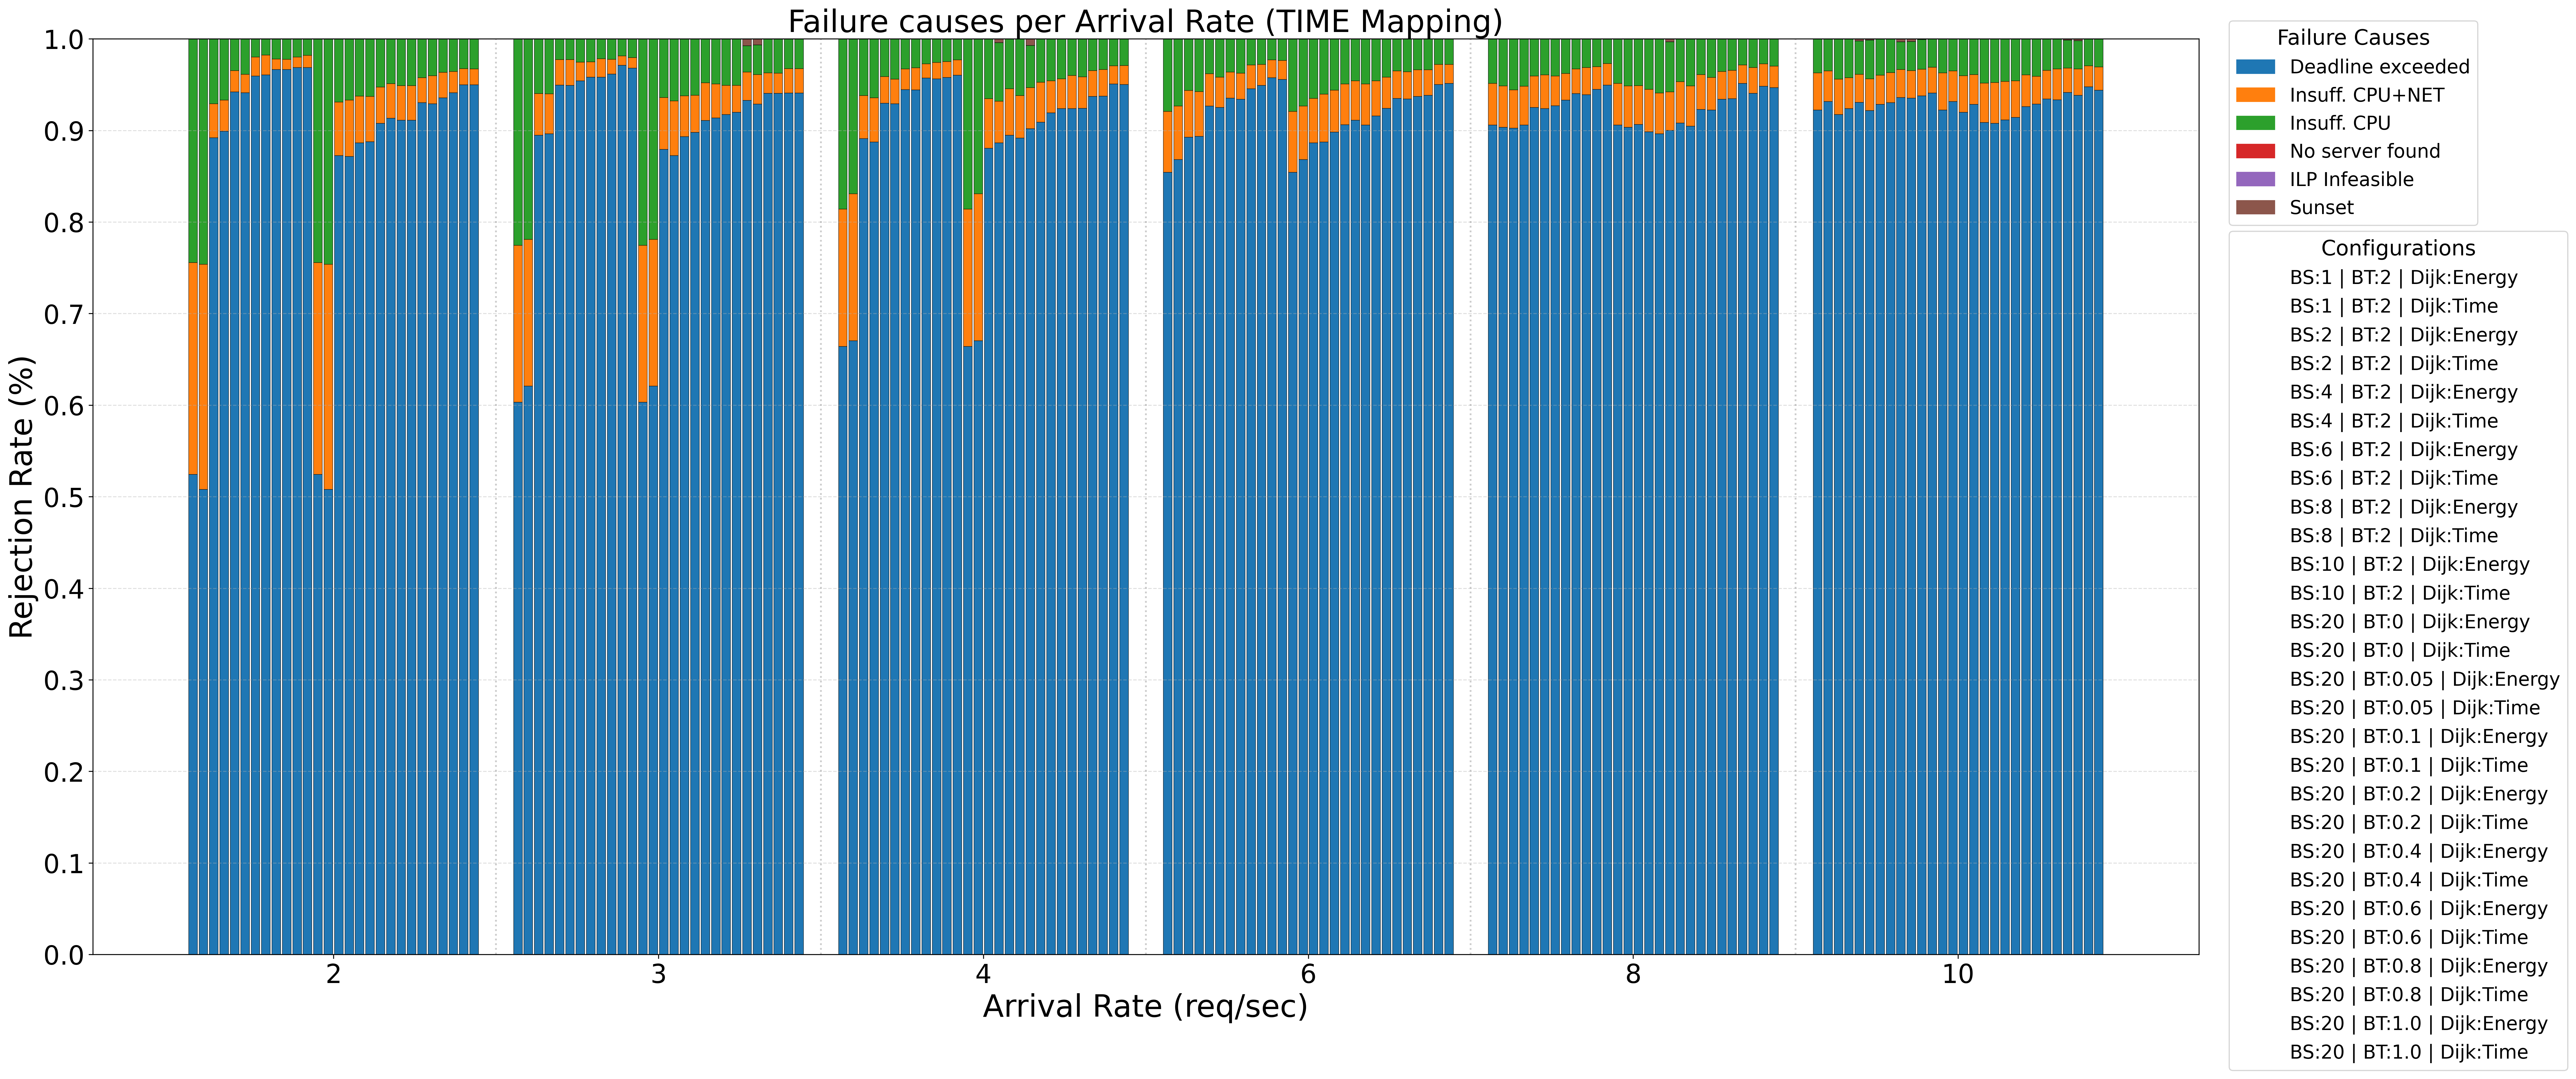
\includegraphics[width=1.3\textwidth]{02_AR_rejection_time.png}}
    \caption{Distribuzione delle Cause di Rigetto sul totale dei task (Configurazione Time).}
    \label{fig:rej_time}
\end{figure}

L'analisi delle cause di scarto (Figure~\ref{fig:rej_energy} e~\ref{fig:rej_time}) conferma che i fallimenti per limiti di risorse (\textit{Rej. CPU} e \textit{Rej. CPU/NET}) risultano marginali, riducendosi ulteriormente all'aumentare del carico. La causa predominante e quasi assoluta del drop dei task è la violazione dei vincoli temporali (\textit{Rej. Deadline}).

\subsection{Scomposizione del Tempo di Risposta (Response Time)}
L'ultima fase si concentra sul disaggregare il tempo di risposta totale nella componente di calcolo (\textit{System Execution}) e in quella di accodamento/instradamento (\textit{Network/Wait Time}).

\begin{figure}[H]
    \makebox[\textwidth][c]{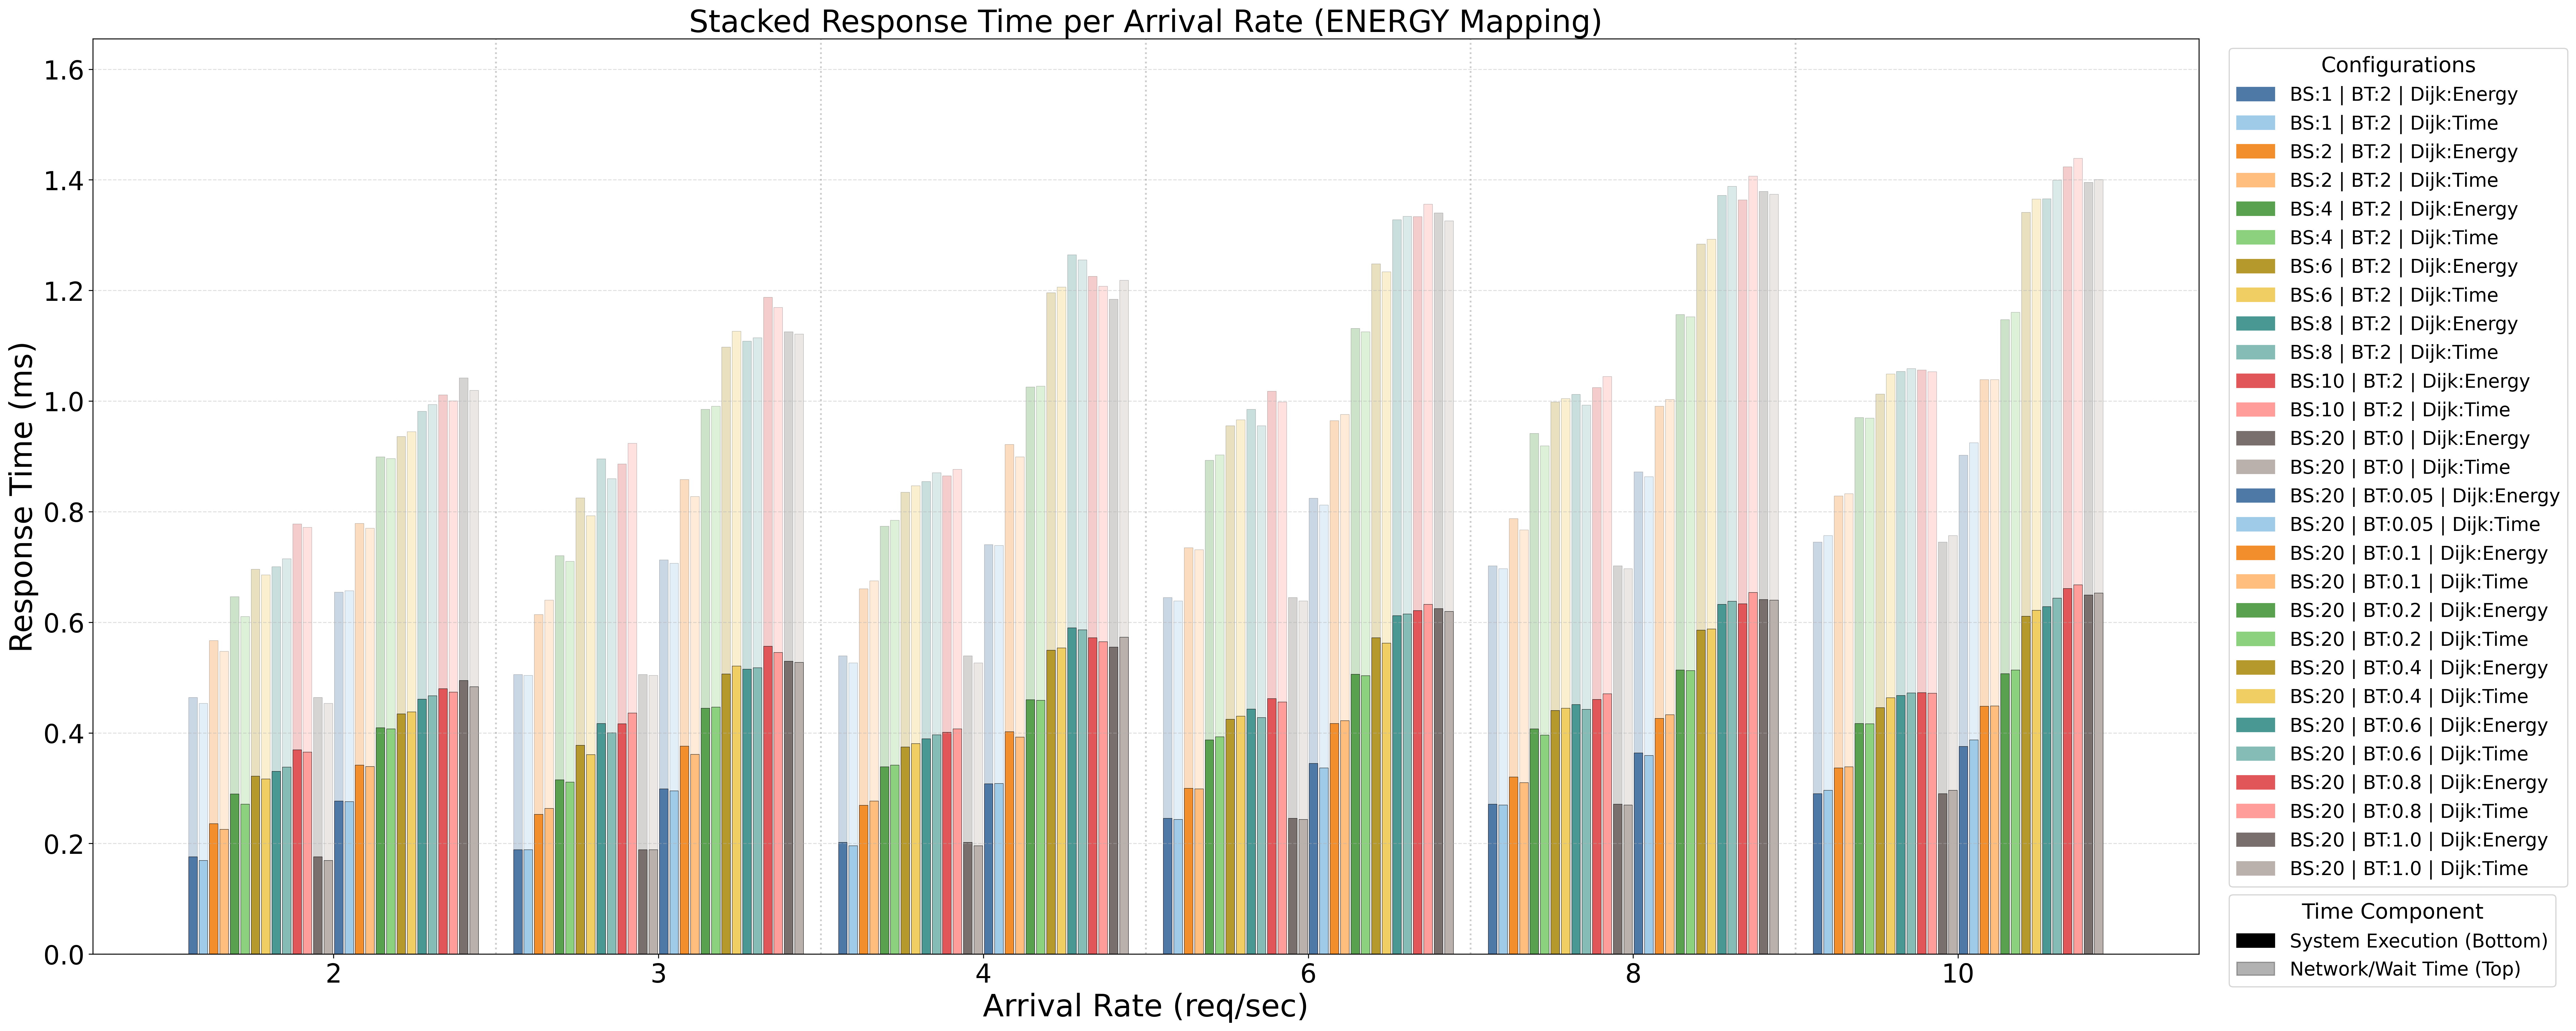
\includegraphics[width=1.3\textwidth]{03_AR_response_energy.png}}
    \caption{Scomposizione del Response Time (Configurazione Energy).}
    \label{fig:response_energy}
\end{figure}

\begin{figure}[H]
    \makebox[\textwidth][c]{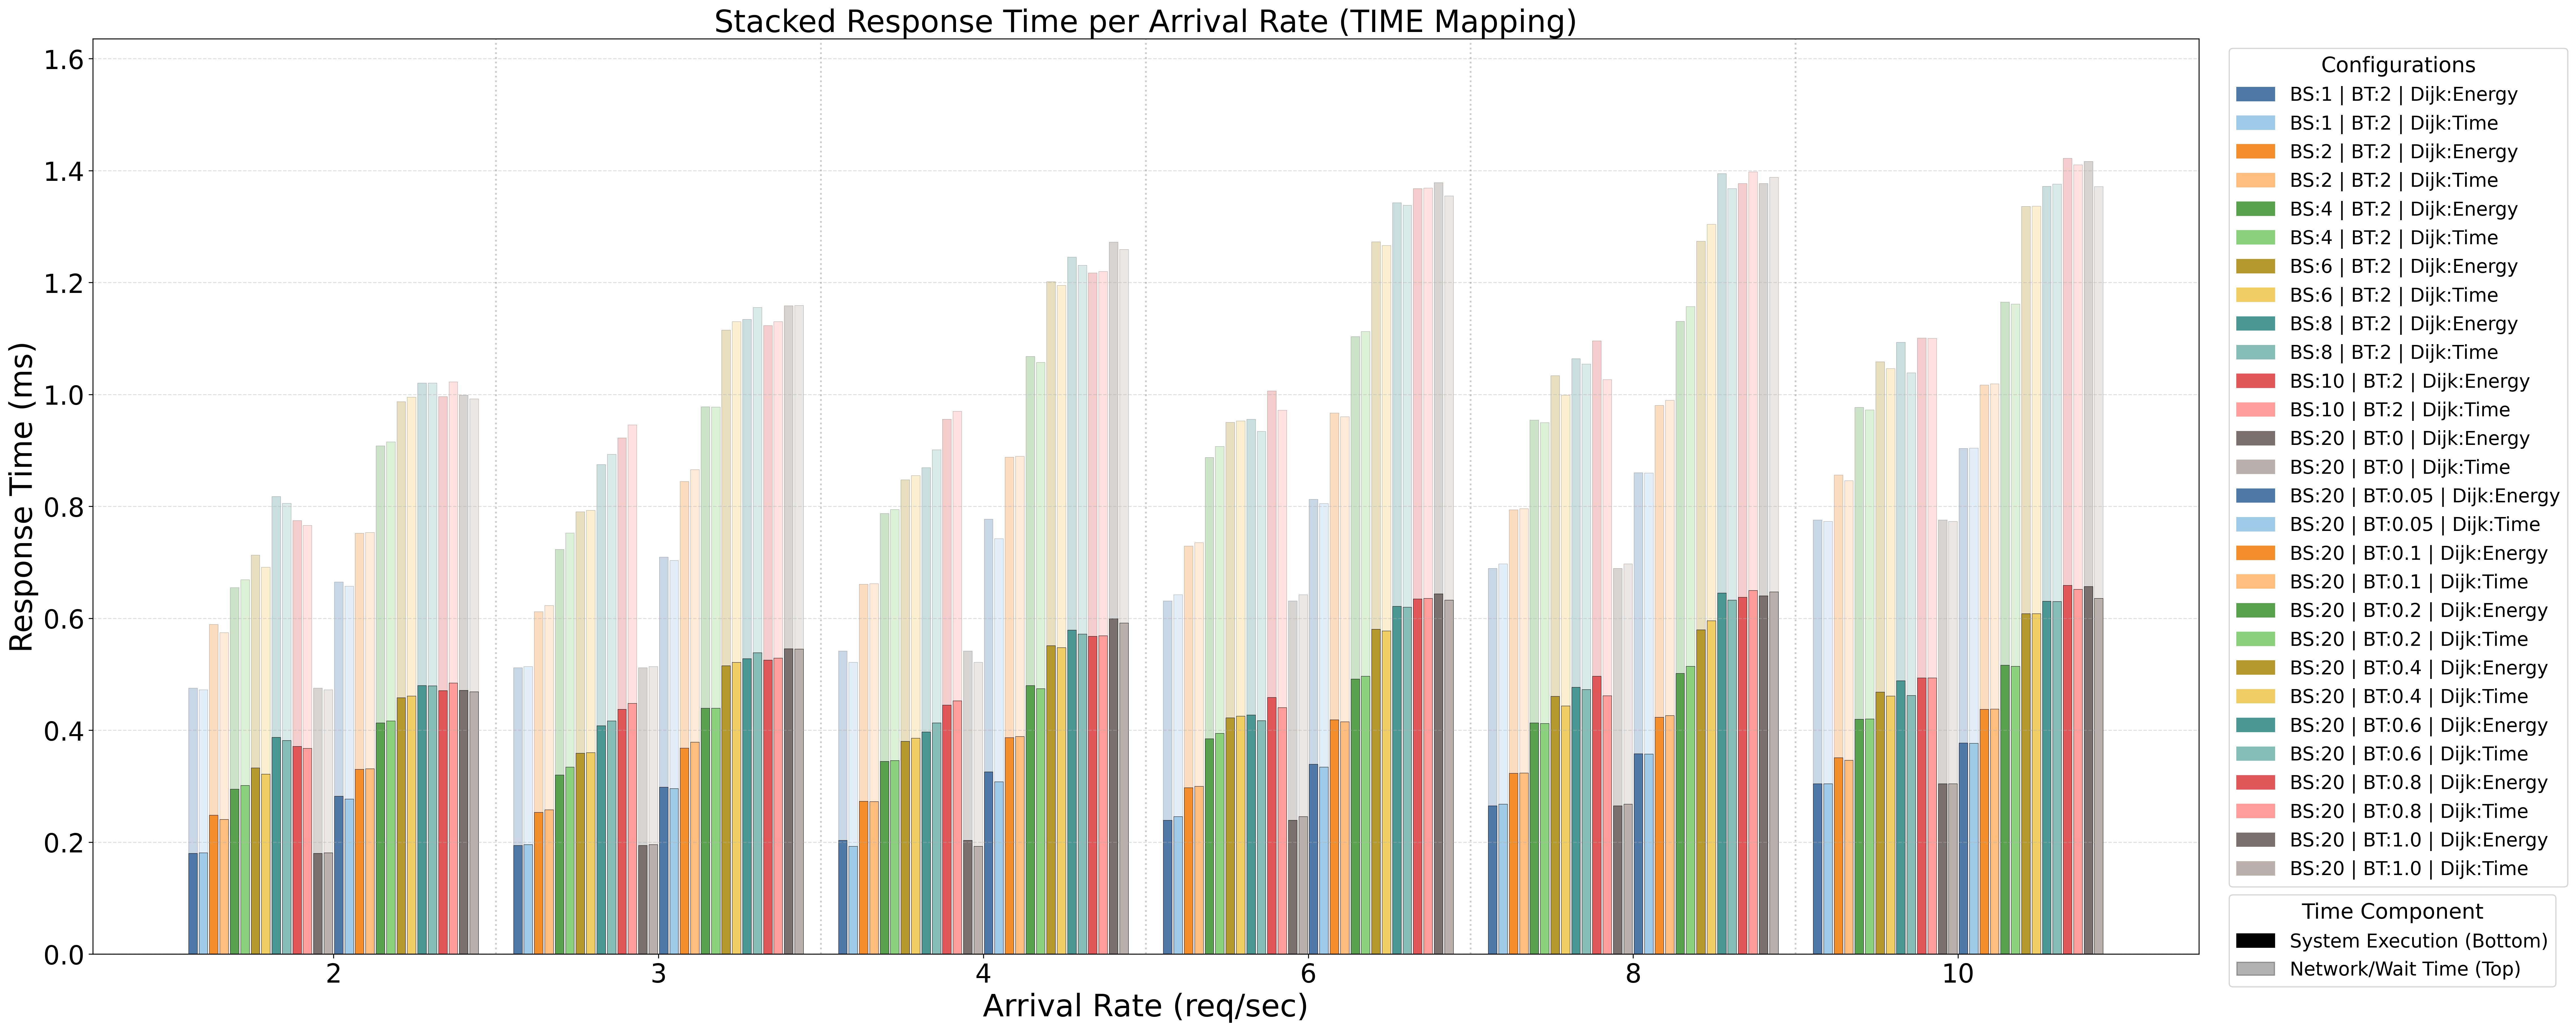
\includegraphics[width=1.3\textwidth]{03_AR_response_time.png}}
    \caption{Scomposizione del Response Time (Configurazione Time).}
    \label{fig:response_time}
\end{figure}


L'andamento dei tempi di risposta totali al variare del carico è illustrato in Figura~\ref{fig:response_energy} (\textit{Energy}) e Figura~\ref{fig:response_time} (\textit{Time}). Per tutte le configurazioni, si osserva un fisiologico incremento della latenza all'aumentare dell'Arrival Rate, guidato dal progressivo accumulo delle richieste nel sistema.

I nuovi grafici smentiscono l'apparente vantaggio prestazionale dei batch più ampi, mostrando chiaramente come l'aggregazione prolungata penalizzi severamente la latenza. Osservando le componenti impilate, si evince che il tempo di esecuzione effettivo del sistema (porzione inferiore scura) si mantiene relativamente stabile. Il drammatico aumento dei tempi di risposta per le configurazioni ad alta capacità (es. $BS=8, 10$ o $20$) è interamente dominato dal tempo di attesa (\textit{Wait Time}, porzione superiore chiara).


\section{Conclusioni}


L'analisi sperimentale ha convalidato la solidità dell'orchestrazione centralizzata ILP in contesti a carico medio-basso. L'utilizzo strutturato del Batching e del Timeout si è rivelato la scelta architetturale più impattante: accumulare richieste destabilizza l'algoritmo. I dati riassuntivi dell'intera simulazione sono aggregati nella Tabella \ref{tab:summary_csv}.

\section{Dati Sperimentali}

\begin{longtable}{ccccccc}
\caption{Tabella Riassuntiva: Valori medi (aggregati per Batch Size e Batch Timeout) al variare dell'Arrival Rate.} \label{tab:summary_csv} \\
\toprule
\textbf{Batch} & \textbf{Batch} & \textbf{Arrival} & \textbf{Success} & \textbf{Rej.} & \textbf{Rej.} & \textbf{Avg Total} \\
\textbf{Size} & \textbf{Timeout} & \textbf{Rate} & \textbf{Rate (\%)} & \textbf{Deadline (\%)} & \textbf{CPU (\%)} & \textbf{Resp. (ms)} \\
\midrule
\endfirsthead

\multicolumn{7}{c}%
{{\bfseries Tabella \thetable\ continuazione dalla pagina precedente}} \\
\toprule
\textbf{Batch} & \textbf{Batch} & \textbf{Arrival} & \textbf{Success} & \textbf{Rej.} & \textbf{Rej.} & \textbf{Avg Total} \\
\textbf{Size} & \textbf{Timeout} & \textbf{Rate} & \textbf{Rate (\%)} & \textbf{Deadline (\%)} & \textbf{CPU (\%)} & \textbf{Resp. (ms)} \\
\midrule
\endhead

\midrule
\multicolumn{7}{r}{{Continua nella pagina successiva...}} \\
\endfoot

\bottomrule
\endlastfoot

        1 & 2.0 & 2 & 89.56\% & 5.39\% & 2.79\% & 0.464 ms \\
        1 & 2.0 & 3 & 87.63\% & 7.31\% & 2.68\% & 0.505 ms \\
        1 & 2.0 & 4 & 84.45\% & 9.78\% & 3.36\% & 0.540 ms \\
        1 & 2.0 & 6 & 65.65\% & 29.30\% & 2.81\% & 0.645 ms \\
        1 & 2.0 & 8 & 51.87\% & 43.70\% & 2.46\% & 0.702 ms \\
        1 & 2.0 & 10 & 40.96\% & 55.10\% & 2.09\% & 0.745 ms \\
        1 & 2.0 & 2 & 90.01\% & 5.47\% & 2.42\% & 0.454 ms \\
        1 & 2.0 & 3 & 88.71\% & 6.81\% & 2.53\% & 0.504 ms \\
        1 & 2.0 & 4 & 85.03\% & 10.03\% & 2.82\% & 0.526 ms \\
        1 & 2.0 & 6 & 66.02\% & 29.27\% & 2.49\% & 0.639 ms \\
        1 & 2.0 & 8 & 51.37\% & 43.66\% & 2.58\% & 0.697 ms \\
        1 & 2.0 & 10 & 40.76\% & 55.08\% & 2.28\% & 0.757 ms \\
        \midrule
        2 & 2.0 & 2 & 56.91\% & 39.01\% & 2.34\% & 0.567 ms \\
        2 & 2.0 & 3 & 56.09\% & 40.33\% & 1.98\% & 0.614 ms \\
        2 & 2.0 & 4 & 53.96\% & 41.05\% & 3.00\% & 0.661 ms \\
        2 & 2.0 & 6 & 52.92\% & 41.95\% & 2.77\% & 0.735 ms \\
        2 & 2.0 & 8 & 45.85\% & 49.50\% & 2.45\% & 0.787 ms \\
        2 & 2.0 & 10 & 36.87\% & 57.63\% & 2.96\% & 0.829 ms \\
        2 & 2.0 & 2 & 57.21\% & 39.12\% & 2.27\% & 0.548 ms \\
        2 & 2.0 & 3 & 57.60\% & 41.61\% & 0.37\% & 0.640 ms \\
        2 & 2.0 & 4 & 54.32\% & 40.56\% & 2.81\% & 0.675 ms \\
        2 & 2.0 & 6 & 52.27\% & 42.33\% & 2.74\% & 0.732 ms \\
        2 & 2.0 & 8 & 45.46\% & 49.50\% & 2.70\% & 0.767 ms \\
        2 & 2.0 & 10 & 36.52\% & 57.99\% & 2.91\% & 0.833 ms \\
        \midrule
        4 & 2.0 & 2 & 37.03\% & 59.32\% & 2.14\% & 0.646 ms \\
        4 & 2.0 & 3 & 34.93\% & 61.30\% & 2.00\% & 0.721 ms \\
        4 & 2.0 & 4 & 33.90\% & 61.67\% & 2.24\% & 0.774 ms \\
        4 & 2.0 & 6 & 32.45\% & 62.60\% & 2.75\% & 0.893 ms \\
        4 & 2.0 & 8 & 32.21\% & 62.65\% & 2.60\% & 0.942 ms \\
        4 & 2.0 & 10 & 30.89\% & 63.49\% & 3.09\% & 0.970 ms \\
        4 & 2.0 & 2 & 37.12\% & 59.51\% & 1.93\% & 0.610 ms \\
        4 & 2.0 & 3 & 34.98\% & 61.02\% & 2.15\% & 0.710 ms \\
        4 & 2.0 & 4 & 34.16\% & 61.69\% & 2.43\% & 0.784 ms \\
        4 & 2.0 & 6 & 32.40\% & 62.75\% & 2.48\% & 0.903 ms \\
        4 & 2.0 & 8 & 31.53\% & 63.29\% & 2.61\% & 0.919 ms \\
        4 & 2.0 & 10 & 30.64\% & 63.65\% & 3.08\% & 0.969 ms \\
        \midrule
        6 & 2.0 & 2 & 30.07\% & 66.73\% & 1.59\% & 0.696 ms \\
        6 & 2.0 & 3 & 27.52\% & 69.30\% & 2.04\% & 0.825 ms \\
        6 & 2.0 & 4 & 26.30\% & 68.99\% & 2.52\% & 0.835 ms \\
        6 & 2.0 & 6 & 24.43\% & 70.53\% & 2.58\% & 0.956 ms \\
        6 & 2.0 & 8 & 23.99\% & 71.27\% & 2.50\% & 0.999 ms \\
        6 & 2.0 & 10 & 23.17\% & 71.69\% & 2.89\% & 1.013 ms \\
        6 & 2.0 & 2 & 30.12\% & 66.85\% & 1.49\% & 0.686 ms \\
        6 & 2.0 & 3 & 27.66\% & 69.07\% & 1.93\% & 0.793 ms \\
        6 & 2.0 & 4 & 26.50\% & 69.57\% & 2.02\% & 0.847 ms \\
        6 & 2.0 & 6 & 24.54\% & 70.90\% & 2.56\% & 0.966 ms \\
        6 & 2.0 & 8 & 23.80\% & 71.45\% & 2.56\% & 1.005 ms \\
        6 & 2.0 & 10 & 23.39\% & 71.27\% & 2.99\% & 1.049 ms \\
        \midrule
        8 & 2.0 & 2 & 26.93\% & 70.54\% & 1.43\% & 0.701 ms \\
        8 & 2.0 & 3 & 24.48\% & 72.60\% & 1.84\% & 0.896 ms \\
        8 & 2.0 & 4 & 22.95\% & 73.71\% & 1.58\% & 0.855 ms \\
        8 & 2.0 & 6 & 21.40\% & 74.48\% & 2.23\% & 0.985 ms \\
        8 & 2.0 & 8 & 20.09\% & 75.49\% & 2.34\% & 1.012 ms \\
        8 & 2.0 & 10 & 19.92\% & 74.89\% & 2.73\% & 1.054 ms \\
        8 & 2.0 & 2 & 27.21\% & 70.26\% & 1.35\% & 0.715 ms \\
        8 & 2.0 & 3 & 24.38\% & 72.75\% & 1.50\% & 0.860 ms \\
        8 & 2.0 & 4 & 23.06\% & 73.43\% & 1.95\% & 0.871 ms \\
        8 & 2.0 & 6 & 21.32\% & 74.49\% & 2.21\% & 0.955 ms \\
        8 & 2.0 & 8 & 20.50\% & 75.01\% & 2.37\% & 0.993 ms \\
        8 & 2.0 & 10 & 19.83\% & 74.92\% & 2.45\% & 1.059 ms \\
        \midrule
        10 & 2.0 & 2 & 26.66\% & 70.86\% & 1.52\% & 0.778 ms \\
        10 & 2.0 & 3 & 22.38\% & 75.17\% & 1.40\% & 0.886 ms \\
        10 & 2.0 & 4 & 20.32\% & 76.58\% & 1.80\% & 0.865 ms \\
        10 & 2.0 & 6 & 18.93\% & 77.45\% & 2.05\% & 1.018 ms \\
        10 & 2.0 & 8 & 18.24\% & 77.52\% & 2.25\% & 1.025 ms \\
        10 & 2.0 & 10 & 17.81\% & 77.61\% & 2.38\% & 1.056 ms \\
        10 & 2.0 & 2 & 26.74\% & 70.78\% & 1.49\% & 0.771 ms \\
        10 & 2.0 & 3 & 22.17\% & 75.53\% & 1.41\% & 0.924 ms \\
        10 & 2.0 & 4 & 20.04\% & 76.61\% & 1.65\% & 0.877 ms \\
        10 & 2.0 & 6 & 19.27\% & 77.45\% & 1.86\% & 0.999 ms \\
        10 & 2.0 & 8 & 18.19\% & 77.52\% & 2.15\% & 1.045 ms \\
        10 & 2.0 & 10 & 17.85\% & 77.41\% & 2.39\% & 1.053 ms \\
        \midrule
        20 & 0.0 & 2 & 89.56\% & 5.39\% & 2.79\% & 0.464 ms \\
        20 & 0.0 & 3 & 87.63\% & 7.31\% & 2.68\% & 0.505 ms \\
        20 & 0.0 & 4 & 84.45\% & 9.78\% & 3.36\% & 0.540 ms \\
        20 & 0.0 & 6 & 65.65\% & 29.30\% & 2.81\% & 0.645 ms \\
        20 & 0.0 & 8 & 51.87\% & 43.70\% & 2.46\% & 0.702 ms \\
        20 & 0.0 & 10 & 40.96\% & 55.10\% & 2.09\% & 0.745 ms \\
        20 & 0.0 & 2 & 90.01\% & 5.47\% & 2.42\% & 0.454 ms \\
        20 & 0.0 & 3 & 88.71\% & 6.81\% & 2.53\% & 0.504 ms \\
        20 & 0.0 & 4 & 85.03\% & 10.03\% & 2.82\% & 0.526 ms \\
        20 & 0.0 & 6 & 66.02\% & 29.27\% & 2.49\% & 0.639 ms \\
        20 & 0.0 & 8 & 51.37\% & 43.66\% & 2.58\% & 0.697 ms \\
        20 & 0.0 & 10 & 40.76\% & 55.08\% & 2.28\% & 0.757 ms \\
        \midrule
        20 & 0.05 & 2 & 62.92\% & 32.58\% & 2.35\% & 0.655 ms \\
        20 & 0.05 & 3 & 59.52\% & 35.96\% & 2.60\% & 0.713 ms \\
        20 & 0.05 & 4 & 56.45\% & 38.98\% & 2.56\% & 0.740 ms \\
        20 & 0.05 & 6 & 52.20\% & 41.43\% & 3.32\% & 0.824 ms \\
        20 & 0.05 & 8 & 46.40\% & 48.71\% & 2.84\% & 0.872 ms \\
        20 & 0.05 & 10 & 38.04\% & 57.08\% & 2.42\% & 0.902 ms \\
        20 & 0.05 & 2 & 63.01\% & 32.34\% & 2.68\% & 0.657 ms \\
        20 & 0.05 & 3 & 59.03\% & 36.27\% & 2.56\% & 0.707 ms \\
        20 & 0.05 & 4 & 56.65\% & 38.64\% & 2.56\% & 0.739 ms \\
        20 & 0.05 & 6 & 52.66\% & 41.65\% & 2.93\% & 0.812 ms \\
        20 & 0.05 & 8 & 46.45\% & 48.66\% & 2.63\% & 0.863 ms \\
        20 & 0.05 & 10 & 37.98\% & 56.92\% & 2.77\% & 0.925 ms \\
        \midrule
        20 & 0.1 & 2 & 51.73\% & 42.90\% & 2.66\% & 0.779 ms \\
        20 & 0.1 & 3 & 46.51\% & 47.67\% & 3.29\% & 0.858 ms \\
        20 & 0.1 & 4 & 45.59\% & 48.78\% & 2.94\% & 0.921 ms \\
        20 & 0.1 & 6 & 41.61\% & 52.35\% & 3.31\% & 0.965 ms \\
        20 & 0.1 & 8 & 39.85\% & 54.22\% & 3.38\% & 0.991 ms \\
        20 & 0.1 & 10 & 35.53\% & 58.10\% & 3.26\% & 1.039 ms \\
        20 & 0.1 & 2 & 50.93\% & 43.49\% & 3.08\% & 0.770 ms \\
        20 & 0.1 & 3 & 47.45\% & 47.45\% & 2.80\% & 0.828 ms \\
        20 & 0.1 & 4 & 44.45\% & 50.07\% & 2.92\% & 0.899 ms \\
        20 & 0.1 & 6 & 41.91\% & 52.09\% & 3.49\% & 0.976 ms \\
        20 & 0.1 & 8 & 39.47\% & 54.15\% & 3.47\% & 1.003 ms \\
        20 & 0.1 & 10 & 35.04\% & 59.18\% & 3.01\% & 1.039 ms \\
        \midrule   
        20 & 0.2 & 2 & 42.82\% & 51.02\% & 3.48\% & 0.899 ms \\
        20 & 0.2 & 3 & 39.27\% & 54.43\% & 3.51\% & 0.985 ms \\
        20 & 0.2 & 4 & 35.96\% & 58.37\% & 3.23\% & 1.025 ms \\
        20 & 0.2 & 6 & 32.27\% & 61.50\% & 3.34\% & 1.132 ms \\
        20 & 0.2 & 8 & 30.53\% & 63.20\% & 3.34\% & 1.157 ms \\
        20 & 0.2 & 10 & 28.69\% & 65.20\% & 3.23\% & 1.147 ms \\
        20 & 0.2 & 2 & 43.59\% & 50.39\% & 3.21\% & 0.896 ms \\
        20 & 0.2 & 3 & 39.06\% & 54.99\% & 3.45\% & 0.991 ms \\
        20 & 0.2 & 4 & 36.23\% & 58.42\% & 3.11\% & 1.027 ms \\
        20 & 0.2 & 6 & 32.11\% & 61.28\% & 3.73\% & 1.125 ms \\
        20 & 0.2 & 8 & 30.37\% & 63.40\% & 3.33\% & 1.153 ms \\
        20 & 0.2 & 10 & 28.78\% & 64.77\% & 3.40\% & 1.161 ms \\
        \midrule
        20 & 0.4 & 2 & 35.92\% & 59.47\% & 2.81\% & 0.936 ms \\
        20 & 0.4 & 3 & 31.33\% & 62.96\% & 3.15\% & 1.097 ms \\
        20 & 0.4 & 4 & 29.19\% & 64.66\% & 3.40\% & 1.196 ms \\
        20 & 0.4 & 6 & 24.46\% & 69.41\% & 2.76\% & 1.248 ms \\
        20 & 0.4 & 8 & 22.61\% & 71.78\% & 3.06\% & 1.284 ms \\
        20 & 0.4 & 10 & 20.72\% & 73.36\% & 3.25\% & 1.341 ms \\
        20 & 0.4 & 2 & 35.82\% & 59.11\% & 2.66\% & 0.945 ms \\
        20 & 0.4 & 3 & 31.56\% & 62.77\% & 3.22\% & 1.126 ms \\
        20 & 0.4 & 4 & 29.49\% & 64.79\% & 3.35\% & 1.206 ms \\
        20 & 0.4 & 6 & 24.46\% & 69.12\% & 3.25\% & 1.234 ms \\
        20 & 0.4 & 8 & 22.66\% & 71.24\% & 3.10\% & 1.292 ms \\
        20 & 0.4 & 10 & 20.86\% & 73.52\% & 3.00\% & 1.365 ms \\
        \midrule
        20 & 0.6 & 2 & 32.87\% & 62.77\% & 2.39\% & 0.982 ms \\
        20 & 0.6 & 3 & 28.41\% & 66.91\% & 2.39\% & 1.108 ms \\
        20 & 0.6 & 4 & 25.16\% & 68.94\% & 3.22\% & 1.264 ms \\
        20 & 0.6 & 6 & 21.03\% & 73.49\% & 2.93\% & 1.328 ms \\
        20 & 0.6 & 8 & 18.91\% & 75.79\% & 2.87\% & 1.372 ms \\
        20 & 0.6 & 10 & 17.19\% & 76.33\% & 3.53\% & 1.366 ms \\
        20 & 0.6 & 2 & 32.86\% & 62.82\% & 2.31\% & 0.994 ms \\
        20 & 0.6 & 3 & 28.60\% & 66.82\% & 2.48\% & 1.115 ms \\
        20 & 0.6 & 4 & 24.94\% & 69.59\% & 2.87\% & 1.255 ms \\
        20 & 0.6 & 6 & 21.21\% & 73.16\% & 3.04\% & 1.334 ms \\
        20 & 0.6 & 8 & 18.94\% & 75.79\% & 2.99\% & 1.389 ms \\
        20 & 0.6 & 10 & 17.23\% & 77.36\% & 2.96\% & 1.399 ms \\
        \midrule
        20 & 0.8 & 2 & 30.73\% & 64.91\% & 2.97\% & 1.012 ms \\
        20 & 0.8 & 3 & 25.93\% & 69.95\% & 2.52\% & 1.188 ms \\
        20 & 0.8 & 4 & 22.91\% & 71.98\% & 2.78\% & 1.226 ms \\
        20 & 0.8 & 6 & 18.62\% & 76.11\% & 2.90\% & 1.334 ms \\
        20 & 0.8 & 8 & 16.77\% & 77.34\% & 2.35\% & 1.364 ms \\
        20 & 0.8 & 10 & 15.19\% & 79.25\% & 2.92\% & 1.424 ms \\
        20 & 0.8 & 2 & 30.62\% & 65.16\% & 2.64\% & 1.001 ms \\
        20 & 0.8 & 3 & 26.17\% & 69.61\% & 2.54\% & 1.169 ms \\
        20 & 0.8 & 4 & 23.04\% & 72.08\% & 2.69\% & 1.208 ms \\
        20 & 0.8 & 6 & 18.54\% & 75.52\% & 2.62\% & 1.356 ms \\
        20 & 0.8 & 8 & 16.67\% & 78.07\% & 2.80\% & 1.407 ms \\
        20 & 0.8 & 10 & 14.96\% & 79.42\% & 2.65\% & 1.439 ms \\
        \midrule
        20 & 1.0 & 2 & 30.16\% & 65.45\% & 2.60\% & 1.042 ms \\
        20 & 1.0 & 3 & 25.56\% & 70.67\% & 2.18\% & 1.126 ms \\
        20 & 1.0 & 4 & 21.16\% & 74.75\% & 2.16\% & 1.184 ms \\
        20 & 1.0 & 6 & 17.29\% & 78.47\% & 2.42\% & 1.340 ms \\
        20 & 1.0 & 8 & 15.20\% & 80.04\% & 2.54\% & 1.379 ms \\
        20 & 1.0 & 10 & 13.93\% & 81.51\% & 2.39\% & 1.395 ms \\
        20 & 1.0 & 2 & 30.28\% & 65.64\% & 2.36\% & 1.020 ms \\
        20 & 1.0 & 3 & 24.95\% & 71.22\% & 2.31\% & 1.121 ms \\
        20 & 1.0 & 4 & 21.19\% & 74.77\% & 2.16\% & 1.218 ms \\
        20 & 1.0 & 6 & 16.98\% & 78.21\% & 2.59\% & 1.326 ms \\
        20 & 1.0 & 8 & 15.25\% & 80.01\% & 2.33\% & 1.374 ms \\
        20 & 1.0 & 10 & 13.89\% & 81.61\% & 2.46\% & 1.401 ms \\
\end{longtable}
\end{document}